\chapter{State of the Art}
\label{cap:estadoDeLaCuestion}
\chapterquote{Who controls the past controls the future.\\Who controls the present controls the past.}{1984 - George Orwell (1949)}

In order to be able to develop a model for stylometric analysis of e-mails for recipient-based personalised writing, the first thing we need to understand is the fundamentals of this communication method. For this reason, in Section \ref{sect:email}, we delve into both the protocols that define it and the specific structure of the Gmail service, since the e-mail account that we analyse and that is used to design the model around the data extracted from it belongs to that service.

Once we have laid the foundations of communication through e-mail and, specifically, the Gmail service, we study how to analyse the wording of the different messages, that is to say, we learn the concepts of the field of study known as stylometry (see Section \ref{sect:compstyl}). Specifically, we also present the research related to e-mails and the most common techniques and metrics used for various purposes.

Finally, for the modelling of a recipient-based custom writing system, we need to understand the functioning of a very popular technique in information retrieval called Latent Semantic Indexing. For this reason, in Section \ref{sect:lsi}, we explain this method in detail, which is used in later chapters.

\section{Electronic Mail}\label{sect:email}
Electronic Mail \citep[Chapter 11]{redhatemail} is a communication service which has been used since 1971 \citep{wikiemail} when the first network e-mail with the text ``QWERTYUIOP'' was sent through ARPAnet (Advanced Research Projects Agency Network, the first network which implements the TCP/IP protocol) with the experimental protocol CYPNET. Nowadays, the messages are delivered by using a client/server architecture. In this way, an e-mail is created by using a client-side mail program. Then, this software sends the message to a server, which will redirect it to the recipient's mail server. From there, the e-mail is delivered to the addressee.

According to \cite{radicati2020email}, e-mail is ``still the most pervasive form of electronic communication for both business and consumer users'' and both the number of e-mail accounts and the amount of messages sent continue to grow. The evolution of worldwide daily e-mail traffic can be seen in Table \ref{tab:dailymail}, where we can observe the huge amount of messages which are sent every day and its evolution over the next four years.

\begin{table}[]
	\centering
	\begin{tabular}{|l|l|l|l|l|l|}
		\hline
		\textbf{Year} & 2020 & 2021 & 2022 & 2023 & 2024 \\ \hline
		\textbf{\begin{tabular}[c]{@{}l@{}}Billions of worldwide e-mails\\ sent/receive per day\end{tabular}} & 306.4 & 319.6 & 333.2 & 347.3 & 361.6 \\ \hline
		\textbf{Percentage of growth} & 4.4 & 4.3 & 4.3 & 4.2 & 4.1 \\ \hline
	\end{tabular}
\caption{Worldwide daily e-mail traffic (2020-2024)}\label{tab:dailymail}
Table extracted from \cite{radicati2020email}.
\end{table}

In order to make the sending of all these messages possible, an Internet standard that extends the format of e-mail messages, and a wide range of network protocols exist for allowing different machines (which often execute distinct operative systems and make use of different mail programs) to share e-mails. In this section, we are going to study this standard, these protocols and the API which is going to be used for reading, sending e-mails and accessing to the user's e-mail data. First of all, we are going to explain the MIME standard (see Section \ref{ssect:mime}) which specifies the format of e-mail messages. Then we are going to explain the main e-mail management protocols, both electronic mail transmission protocol (such as Simple Mail Transfer Protocol, which is explained in Section \ref{ssect:smtp}) and message access protocol (such as Post Office Protocol and Internet Message Access Protocol, which are studied in Sections \ref{ssect:pop} and \ref{ssect:imap}, respectively).

In spite of being a mail server-independent solution, as we will see, we are going to find security issues which are going to hinder our user's e-mail data access. These trials come from the automatic server access. For this reason, Gmail API is going to be introduced (see Section \ref{ssect:gmailapi}) and, finally, the assessment of the advantages and disadvantages of making use of the e-mail protocols or the Gmail API is discussed (see Section \ref{ssect:protvsapi}).

\subsection{MIME} \label{ssect:mime}
To be able to automatically create messages and read the body of the e-mails, it is essential to understand what the MIME standard consists in. Hence, in this section we are going to give a general idea about this.

MIME, whose acronym stands for Multipurpose Internet Mail Extensions, is an Internet standard for the exchange of several file types (text, audio and video among others) which provides support to text with characters other than ASCII, non-text attachments, body messages with numerous parts (known as multi-part messages) and headers information with characters other than ASCII. It is defined in a series of Request For Comments (RFC): RFC 2045 \citep{rfc2045}, RFC 2046 \citep{rfc2046}, RFC 2047 \citep{rfc2047}, RFC 2049 \citep{rfc2049}, RFC 2077 \citep{rfc2077}, RFC 4288 \citep{rfc4288} and RFC 4289 \citep{rfc4289}.

Virtually all e-mails written by people on the Internet and a considerable proportion of these automatically generated messages are transmitted in MIME format via SMTP (see Section \ref{ssect:smtp}). Internet e-mail messages are so closely associated with SMTP and MIME that they are usually called SMTP/MIME messages.

The content types defined by the MIME standard are of great importance also outside the context of e-mails. Examples of this are some network protocols such as HTTP from the Web. HTTP requires data to be transmitted in an e-mail-type message context although the data may not be an e-mail itself.

Nowadays, no e-mail program or Internet browser can be considered complete if it does not accept MIME in its various facets (text and file formats). 

In this section we will learn about the MIME type nomenclature (see Section \ref{sssect:MIMEtype}), which is necessary for being able to exchange several file types. Then, we will illustrate the MIME structure of an e-mail, consisting of MIME headers (see Section \ref{sssect:MIMEheaders}) and, finally, two common MIME message encoding (base64 and quoted-printable) are explained (see Sections \ref{sssect:base64} and \ref{sssect:quot-p}, respectively).

\subsubsection{Type Nomenclature}\label{sssect:MIMEtype}

Each data type has a different name in MIME. These names follow the format: type/subtype (both type and subtype are strings), in such a way that the first denotes the general data category and the second the specific type of that information. The values the type can take are:

\begin{itemize}
	\item\textit{text}: means that the content is simple text. Subtypes like \textit{html}, \textit{xml} and \textit{plain} can follow this type.
	\item\textit{multipart}: indicates that the message has numerous parts with independent data. Subtypes like \textit{form-data} and \textit{digest} can follow this type.
	\item\textit{message}: it is used to encapsulate an existing message, for example when we want to reply a e-mail and add the previous message. Subtypes like \textit{partial} and \textit{rfc822} can follow this type.
	\item\textit{image}: means that the content is an image. Subtypes like \textit{png}, \textit{jpeg} and \textit{gif} can follow this type.
	\item\textit{audio}: indicates that the content is an audio. Subtypes like \textit{mp3} and \textit{32kadpcm} can follow this type.
	\item\textit{video}: denotes that the content is an video. Subtypes like \textit{mpeg} and \textit{avi} can follow this type.
	\item\textit{application}: it is used for application data that could be binary. Subtypes like \textit{json} and \textit{pdf} can follow this type.
	\item\textit{font}: means that the content is a file which defines a font format. Subtypes like \textit{woff} and \textit{ttf} can follow this type.
\end{itemize}

\subsubsection{MIME headers} \label{sssect:MIMEheaders}

MIME has several headers which appear in all e-mails sent with this standard. The most important of them are the following:

\begin{itemize}
	\item\textit{Content-Type}: the value of this header is the type and subtype of the message with the same structure that we have explained before. For example, if we have the header \textit{Content-Type: text/plain}, it means that the message is a plain text. The use of the type \textit{multipart} makes the creation of messages with parts and subparts organized in a tree structure (in which leaf nodes can belong to any type and the rest of them can belong to any multipart subtype variety) possible \citep[Section 7.2]{rfc1341}. A feasible composition of a message with a part with plain text and other non-text parts could be constructed by using \textit{multipart/mixed} as the root node like in Figure \ref{fig:content-type}. Indeed, in the example of Figure \ref{fig:content-type} we can observe the use of \textit{multipart/alternative} for a message which contains the body both in plain text and in html text. Other different e-mails constructions are possible (like forwarding with the original message attached by using \textit{multipart/mixed} with a \textit{text/plain} part and a \textit{message/rfc822} part) thanks to the tree structure of the \textit{Content-type} header.
	
	Another important detail, that we can observe in the example in Figure \ref{fig:content-type}, is the fact that each node of the tree structure of the e-mails is visited and showed following the pre-order traversal.
	
	\begin{figure}[t]
		\centering%
		\centerline{\includegraphics[width = 1.2\textwidth]{Imagenes/Bitmap/tree-content-type.png}}%
		\caption{MIME types tree structure of an e-mail example}%
		\label{fig:content-type}
	\end{figure}
	\item\textit{Content-Disposition}: this header is used to indicate the presentation style of the part of the message. There are two ways to show the part: \textit{inline} content-disposition (which means that the content must be displayed at the same time as the message) and \textit{attachment} content-disposition (the part is not displayed at the same time as the message and it requires some form or action from the user to see it). Furthermore, this header also provides several fields for specifying other type of information about the content, such as the name of the file and the creation or modification date. The following example is taken from RFC 2183 \citep{rfc2183} and, as we will explain after the example, it does not match with the syntax of this same header in the example that we can see in the last part of the example message of Figure \ref{fig:content-type}:
	\begin{lstlisting}
	Content-Disposition: attachment; filename=genome.jpeg;
	modification-date="Wed, 12 Feb 1997 16:29:51 -0500";
	\end{lstlisting}
	As we have said, this syntax is different from the one used in the e-mail example of Figure \ref{fig:content-type}. This results from the fact that, in HTTP, the header we find in that figure (\textit{Content-Disposition: attachment}) is usually used for instructing the client to show the response body as a downloadable file. As we can observe, it has a \textit{filename} field which is used for establishing the default file name when the user is going to download it.
	
	\item\textit{Content-Transfer-Encoding}: when we want to send some files in a message, sometimes they are represented as 8-bit character or binary data, which are not allowed in some protocols. On this account, it is necessary to have a standard that indicates how we should re-encode such data into a 7-bit short-line format. The Content-Transfer-Encoding header \citep[Section 5]{rfc1341} will tell the client which transformation has been used for being able to transport that data. Therefore, and for lack of a previous standard which states a single Content-Transfer-Encoding mechanism, the possible values which specify the type of encoding are: \textit{'base64'} (see Section \ref{sssect:base64}), \textit{'quoted-printable'} (see Section \ref{sssect:quot-p}), \textit{'8bit'}, \textit{'7bit'}, \textit{'binary'} and \textit{'x-token'}. All these values are not case sensitive. If this header does not exist, we can assume that the value of this header is \textit{'7bit'}, which means that the body of the message is already in a seven-bit mail-ready representation, in other words, all the body of the message is represented as short lines of US-ASCII data. Despite \textit{'8bit'}, \textit{'7bit'} and \textit{'binary'} indicate that the content has not been transformed, they are useful for knowing the kind of encoding that the data has. This header will generally be omitted when the Content-Type has the \textit{multipart} or \textit{message} type (as it happens in the message example of Figure \ref{fig:content-type}), because it also admits the last three types we have mentioned.
	
	It is common to add another header (as we can see in Figure \ref{fig:content-type}) called \textit{charset}, the value of which represents the original encoding of data so the client is able to decode it.
\end{itemize}

\subsubsection{Base64 encoding} \label{sssect:base64}
As we have studied when we learnt how the MIME headers (see Section \ref{sssect:MIMEheaders}) are, we can find e-mail whose content encoding is base64. Base64 \citep{rfc4648} is a group of reversible binary-to-text encoding schemes which represent binary data as a sequence of ASCII printable characters. It makes use of a radix-64 to translate each character, because 64 is the highest power of two than can be represented using only printable ASCII characters. Indeed all the Base64 variants (like base64url) utilise the characters range A-Z, a-z and 0-9 in that order for the first 62 digits, but the chosen symbol for the last two digits are very different between them. In particular, the MIME (see Section \ref{ssect:mime}) specification, established in RFC 2045 \citep{rfc2045}, describes base64 based on  Privacy-enhanced Electronic Mail (PEM) protocol (defined by \cite{rfc1421}, \cite{rfc1422}, \cite{rfc1423} and \cite{rfc1424}), which means that the last two characters are '+' and '/', and the symbol '=' is used for output padding suffix. In the same way, MIME does not stablish a fixed size for the base64 encoded lines, by contrast it specifies a maximum size of 76 characters.

If we try to apply standard base64 in a URL encoder, it will translate the characters '+' and '/' to its hexadecimal representation ('+' = '\%2B' and '/' = '\%2F'). This will cause a conflict in heterogeneous systems or if we use it in data base storage, because of the character '\%' produced by the encoder (it is a special symbol of ANSI SQL). This is why modified Base64 for URL variants exists (such as base64url in \cite{rfc4648}), where the '=' character has no usefulness and the '+' and '/' symbols are replaced by '-' and '\_' respectively. Besides it has no impact on the size of encoded lines.

\subsubsection{Quoted-printable enconding} \label{sssect:quot-p}
Other reversible binary-to-text encoding that could be used in the content of a MIME message is the quoted-printable encoding \citep{rfc1521}. Making use of printable characters (such as alphanumeric and '=') proved capable of transmitting 8 bit data over a 7 bit protocol. Unlike base64, if the original message is mostly composed of ASCII characters, the encoded text is readable and compact.

Each byte can be represented via two hexadecimal characters. On this basis, the '=' symbol followed by two hexadecimal digits are enough to encode all the characters except the printable ASCII ones and the end of line. For example, if we want to represent the $12^th$ ASCII character we can encode it as '=0C' or if the equality symbol (whose decimal value is 61) is in our original message, it could be encoded as '=3D' (note that despite being a printable ASCII character it must be encoded as it is a special character in this encoding). This is how quoted-printable encodes the different characters.

In respect of the maximum line size, as it happens with the MIME specification of the base64 (see Section \ref{sssect:base64}), it has a length of 76 characters each encoded line. To achieve this goal and still be able to decode the text getting the original message, quoted-printable adds \textit{soft line breaks} at the end of the line consisting of the '=' symbol and it does not modify the encoded text.

\subsection{Simple Mail Transfer Protocol} \label{ssect:smtp}

Simple Mail Transfer Protocol (also known as SMTP) is a network connection-oriented communication protocol used for the exchange of e-mail messages. It was originally defined by \cite{rfc821} (for the transfer) and by \cite{rfc822} (for the message). It is currently defined by \cite{rfc5321} and \cite{rfc5322}. However, this protocol has some limitations when it comes to receiving messages on the destination server. For this reason, this task is intended for other protocols such as the Internet Message Access Protocol (see Section \ref{ssect:imap}) or the Post Office Protocol (refer to Section \ref{ssect:pop}), and SMTP is used specifically to send messages.

Making use of SMTP, an e-mail is ``pushed'' from one mail server to another (next-hop mail server) until it reaches its destination. The message is not routed according to the message recipients specified during the client's connection to the SMTP server, but from the destination mail server. Thanks to the fact that this protocol has a feature to initiate mail queue processing, an intermittently connected mail server can extract messages from another remote server when necessary.

\subsection{Post Office Protocol} \label{ssect:pop}

Post Office Protocol (also known as POP) is an application protocol (in OSI Model) for obtaining e-mails stored in a remote Internet server called POP server. It was originally defined by \cite{rfc918} (it was POP version 1, also known as POP1). Current POP version (POP3, in general when we talk about POP we refer to this version) is detailed by \cite{rfc1939}.

POP3 was designed for receiving e-mails. Using POP3, users with intermittent or very slow Internet connections (such as modem connections) can download their e-mail while online and check it later even when offline. The general operation is: a client using POP3 connects, gets all messages, stores them on the user's computer as new messages, deletes them from the server, and finally disconnects. However some mail clients include the option to leave messages on the server. They use the order UIDL (Unique IDentification Listing) which, unlike most POP3 commands, does not identify messages depending on their mail server ordinal number. This results from the fact that the mail server ordinal number creates problems when a client tries to leave messages on the server, since messages with numbers change from one connection to the server to another. Accordingly, a server which makes use of UIDL, assigns a unique and permanent character string to each message. Thus, when a POP3-compatible mail client connects to the server, it uses the UIDL command to map the message identifier. This way the client can use that mapping to determine which messages to download and which to save at the time of downloading.

Like other old Internet protocols, POP3 used a signature mechanism without encryption. The transmission of POP3 passwords in plain text still occurs. Nowadays POP3 has various authentication methods that offer a diverse range of levels of protection against illegal access to users' mailboxes.

The advantage over other protocols is that between server-client you do not have to send so many commands for communication between them. The POP protocol also works properly if you do not use a constant connection to the Internet or to the network that contains the mail server.

\subsection{Internet Message Access Protocol} \label{ssect:imap}

Internet Message Access Protocol (also known as IMAP) is an application protocol, designed as an alternative to Post Office Protocol (see Section \ref{ssect:pop}) in 1986, which allows the access to stored messages in an Internet server. As with the Post Office Protocol, with IMAP you can access your e-mail from any computer with an Internet connection. The current version of IMAP (IMAP version 4 review 1, or IMAP4rev1) is defined by \cite{rfc3501}.

In contrast to Post Office Protocol, IMAP allows multiple clients to manage the same mailbox. This fact results from the main differences between these two protocols: IMAP does not remove e-mail from the server until the client specifically requests it (as POP removes them by default, it is impossible to access them from another device which has not downloaded the messages) and it does not download the messages to the user's computer (clients may optionally store a local copy of them). This last property gives raise to several advantages with regard to Post Office Protocol: the immediate notification of the arrival of a mail (due to it works in permanent connection mode) while POP checks if there are new e-mails every few minutes (which causes an appreciable rise in traffic and in the time the user has to wait to send a request to the server, because it is necessary to complete the download of all new messages first), it is possible to create shared folders with other users (it depends on the mail server), the e-mails do not take up memory in the user's local device while POP downloads them regardless of whether they are going to be read or not (effectively IMAP has to download a message when it is going to be read, but they are temporary files and only the e-mail headers are downloaded to manage the mailbox) and it allows the user to manage folders, templates and drafts in server in addition to be able to search a mail from keywords.

\subsection{Gmail API}\label{ssect:gmailapi}
Gmail is a free e-mail service developed by the company Google. Users can access Gmail on the web itself and through third-party programs that synchronize e-mail content via POP or IMAP protocols. It also has a mobile application to manage the user's e-mail. Gmail began as a limited beta version on April 1, 2004 and completed its testing phase on July 7, 2009. As stated by \cite{gmailbbc}: ``Gmail is the world's most popular e-mail service with 1.4 billion users''.

As we will see in Section \ref{ssect:protvsapi}, due to the automatic server access, directly using the communication protocol for electronic mail transmission (SMTP) and for retrieving e-mail messages from a mail server (POP or IMAP) will cause us security problems in accessing the user's e-mail data. For this reason, we are going to make use of Gmail API, that we will study in this Section. Thus, in Section \ref{sssect:oauth} we are going to study the necessary protocol for accessing the Gmail API and consequently for being able to get into the user's e-mail data. Further on, we will require a resource (like a programming object) we can work with and represent all the Gmail structure (see Section \ref{sssect:usersres}). Once we count on this general resource, we have the necessary tools to be able to understand and handle the internal architecture of the Gmail API and the different means it provides in order to achieve our goal. Therefore, in Sections \ref{sssect:labres} to \ref{sssect:drafts} we are going to delve into the essential resources for our purpose: labels, messages, threads and drafts.

Finally, as this API is not the only means of accessing the user's mail data (we have studied other ways in previous sections), we will end with a brief description about the API usage limits (in Section \ref{sssect:apilimits}) to assess its use with respect to other methods of e-mail access.

\subsubsection{OAuth 2.0 Protocol}\label{sssect:oauth}
Open Authorization or OAuth \citep{oauth} is an open standard which allows simple authorization flows for web services or applications. It is a protocol defined in \cite{rfc6749} which allows the site's users to share their information with another site without providing their full identity. This mechanism is used by companies like Google, Facebook, Twitter and Microsoft to allow users to share information about their accounts with third-party applications or websites.

Gmail API, as it also happens in the case of other Google APIs, uses OAuth 2.0 protocol \citep{oauthforgoogle} to handle authentication and authorization. It will provide us a secure and trusted login system to access the user's Gmail data.

The basic working process of OAuth 2.0 protocol can bee seen in Figure \ref{fig:oauth}. As we can observe, at first our application carries out a request in which it sends a token. This token includes, among other things, a credential, which helps Google Servers  to identify the application, and a list of OAuth 2.0 Scopes \citep{oauth-scopes-google}, which are a ``mechanism  in OAuth 2.0 to limit an application's access to a user's account. An application can request one or more scopes. This information is then presented to the user in a consent screen, and the access token issued to the application will be limited to the scopes granted'' \citep{oauth-scopes}. We will use the Gmail API OAuth 2.0 Scope which allows us to read, compose, send, and delete e-mails.

Once the user has logged in the Gmail account (authentication) and accepted all the necessary permissions that our application needs (authorization), our process receives an authorization code which is going to be exchanged for an access token \citep{oauth-exchange}. Then, we will be in possession of the OAuth 2.0 credentials for the user \citep{oauth2.credentials} which we are going to use for accessing the user's Gmail account.

\begin{figure}[h]
	\centering%
	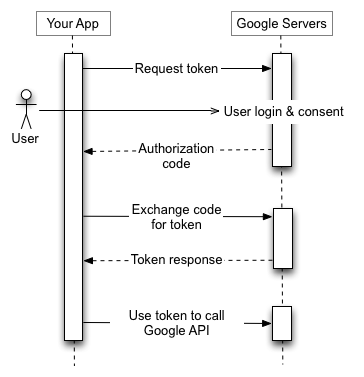
\includegraphics[width = 0.5\textwidth]{Imagenes/Bitmap/webflow.png}%
	\caption{OAuth 2.0 for Web Server Applications and Installed Applications.}%
	Image extracted from \cite{oauthforgoogle}
	\label{fig:oauth}
\end{figure}

\subsubsection{Users resource}\label{sssect:usersres}
At this point, with the OAuth 2.0 credentials, we are able to call the Gmail API. For this purpose, it is necessary to construct a resource \citep[/v1/reference]{gmailAPI} for interacting with the API. As we will see later, this resource will lead us to manage e-mails, drafts, threads and everything we will like to do with the user's Gmail data.

By using the OAuth 2.0 credentials, we are able to get in contact with the Google Servers and request what is known as users resource \citep[/v1/reference/users]{gmailAPI}, which holds all the necessary resources for our task, such as labels (see Section \ref{sssect:labres}), messages (see Section \ref{sssect:msgres}), threads (see Section \ref{sssect:threads}) and drafts (see Section \ref{sssect:drafts}). In practice, the users resource has instance methods which get in contact with Google Servers and return these other Gmail API resources that we are going to need (the methods' names are \textit{labels()}, \textit{messages()}, \textit{threads()} and \textit{drafts()}, respectively). Now, in next sections, we are going to explain all the resources we can create with the user resource.

\subsubsection{Labels resource}\label{sssect:labres}
As we have seen in the explanation of the users resource (Section \ref{sssect:usersres}), we can obtain the labels resource \citep[/v1/reference/users/labels]{gmailAPI} by invoking \textit{labels()} instance method of our users resource. It manages the entire set of our e-mail labels, which  categorize messages and threads within the user's mailbox.

Labels resource is an object which allows us to access to the different e-mail labels of the user, such as \textit{INBOX}, \textit{UNREAD} and \textit{SENT}. With the labels resource methods, we can obtain each of these ``user's labels'' which have a dictionary structure and their representation is what we can observe hereunder:

\begin{python}
	{
		'id' : string, # The immutable identifier of the label
		'name' : string, # The display name
		# The visibility of messages in the Gmail web interface
		'messageListVisibility' : string,
		'labelListVisibility' : string, # The visibility of label
		# The owner type of the label ('system' or 'user')
		'type' : string,
		# Total number of messages with the label
		'messagesTotal' : integer,
		# Number of unread messages with the label
		'messagesUnread' : integer,
		# Total number of threads with the label
		'threadsTotal' : integer,
		# Number of unread threads with the label
		'threadsUnread' : integer,
		'color' : {
			# Text color of the label, represented as hex string
			'textColor' : string,
			# Background color represented as hex string #RRGGBB
			'backgroundColor' : string 
		}
	}
\end{python}

The important fields we are going to need are the \textit{name}, the \textit{type} and the number of total messages and threads with the label (which are \textit{messagesTotal} and \textit{threadsTotal} fields, respectively). Labels with \textit{system} type, such as \textit{INBOX}, \textit{SENT}, \textit{DRAFTS} and \textit{UNREAD}, are internally created and cannot be added, modified or deleted.

\subsubsection{Messages resource}\label{sssect:msgres}
In most of the operations we are going to execute, the correct management of messages will be essential. Therefore, knowing how the e-mails are represented in Gmail API and how to use them is imperative to understand how to work with this API. For this reason, in this section we are going to delve into the messages resource \citep[/v1/reference/users/messages]{gmailAPI} of the Gmail API. As we saw in Section \ref{sssect:usersres}, we can access to this resource by invoking the \textit{messages()} instance method when we have a users resource.

As with the labels resource, the messages resource manages the set of all messages of the user's e-mail. With the messages resource methods, we can obtain each of these ``user's messages'' which, regardless of which programming language is used, have a dictionary structure and their representation is what we can see down below:

\begin{python}
	{
		'id' : string,
		'threadId' : string,
		'labelIds' : [ string ],
		'snippet' : string,
		'historyId' : unsigned long,
		'internalDate' : long,
		'payload' : {
			'partId' : string,
			'mimeType' : string,
			'filename' : string,
			'headers' : [
			{
				'name' : string,
				'value' : string
			}
			],
			'body' : {
				'attachmentId' : string,
				'size' : integer,
				'data' : bytes
			},
			'parts' : [ (MessagePart) ]
		},
		'sizeEstimate' : integer,
		'raw' : bytes
	}
\end{python}

The more important keys of this data structure for this work are:
\begin{itemize}
	\item\textit{id}: an immutable string which identifies the message.
	\item\textit{threadId}: we will explain the thread resource in Section \ref{sssect:threads} and we will see that a thread is composed of different messages that share common characteristics. The value of this field is a string which represent the identifier of the thread the message belongs to.
	\item\textit{labelIds}: a list of the identifiers of labels (see Section \ref{sssect:labres}) applied to the message.
	\item\textit{payload}: as we can see in the resource representation above, it has a dictionary data structure. The \textit{payload} field is the parsed e-mail structure in the message parts. The more important keys of the \textit{payload} field are:
	\begin{itemize}
		\item\textit{mimeType}: the MIME type (see the explanation of \textit{Content-Type} header in Section \ref{sssect:MIMEheaders}) of the message part.
		\item\textit{headers}: a list of headers. It contains the standard RFC 2822 \citep{rfc2822} e-mail headers such as \textit{To}, \textit{From}, \textit{Subject} and \textit{Date}. Each header has a \textit{name} field, which is the name of the header (for example \textit{From}), and a \textit{value} field, which is the value of the header (following the same example as with the \textit{name} field, \textit{example@gmail.com} could be the value).
		\item\textit{parts}: a list which contains the different MIME message child parts (we have gone into it in depth in the Section \ref{ssect:mime}).
		\item\textit{body}: a dictionary structure which contains the body data of this part (see Section \ref{ssect:mime}) in case it does not contain MIME message parts (otherwise it will be empty). This structure should not be confused with an attached file. Each MIME part contains a body property regardless of MIME type of the part.
	\end{itemize}
	\item\textit{raw}: the entire e-mail message in an RFC 2822 \citep{rfc2822} formatted and base64url (see Section \ref{sssect:base64}) encoded string.
\end{itemize}

\subsubsection{Threads resource}\label{sssect:threads}
When we access to our inbox, we are actually seeing the inbox threads instead of the messages resource. Every message, even if it is an only e-mail without a reply, is enclosed in a thread resource \citep[/v1/reference/users/threads]{gmailAPI} which is essentially a list, perhaps unitary, of messages resources. In fact, as we can observe in the following resource representation, each thread (which can be obtained thanks to the threads resource due to it manages the entire set of threads of a user's e-mail), in its dictionary structure, has a list of messages resources:

\begin{python}
	{
		'id' : string, # The identifier of the thread
		'snippet' : string, # A short part of the text
		'historyId' : unsigned long,
		'messages' : [ users.messages resource ]
	}
\end{python}

\subsubsection{Drafts resource}\label{sssect:drafts}
The last Gmail API resource we will study is the most easy to understand after knowing all the structures related with e-mails that we have explained in the above sections: the drafts resource \citep[/v1/reference/users/drafts]{gmailAPI}. Its representation is very simple:

\begin{python}
	{
		'id' : string # The immutable identifier of the draft
		'message' : users.messages resource
	}
\end{python}

As we can observe, a draft is virtually a messages resource with an identifier. Indeed, in order to create a new draft with the \textit{DRAFT} label we must create a MIME message (see Section \ref{ssect:mime}) as we have to do when we want to send a new e-mail by using the \textit{send} messages resource method.

\subsubsection{API Usage Limits} \label{sssect:apilimits}
One factor to be taken into account is the limitations of the Gmail API \citep[/v1/reference/quota]{gmailAPI} which could become a drawback in the application development. It has a limit on the daily usage and on the per-user rate. In order to measure the usage rate, ``quota units'' are defined depending on the method invoked (main methods of each resource are explained in Section \ref{sect:gmailapitech}). In Table \ref{tab:quotaUnits} we can consult the value of some methods in quota units (we have selected the most important methods for our purpose, for the quota units of other methods it is recommended to refer to \cite[/v1/reference/quota]{gmailAPI}).

\begin{table}[h]
	\centering
	\begin{tabular}{|l c r|}
		\hline
		\textbf{Method} & \textbf{Where the method is explained} & \textbf{Quota units} \\
		\hline\hline
		\textit{getProfile} & \ref{ssect:userres} & 1\\ \hline
		\textit{labels.get} & \ref{ssect:labres} & 1\\ \hline
		\textit{messages.get} & \ref{ssect:msgres} & 5\\ \hline
		\textit{messages.list} & \ref{ssect:msgres} & 5\\ \hline
		\textit{messages.send} & \ref{ssect:msgres} & 100\\ \hline
		\textit{threads.get} & \ref{ssect:threads} & 10\\ \hline
		\textit{threads.list} & \ref{ssect:threads} & 10\\ \hline
		\textit{drafts.create} & \citep[/v1/reference/users/drafts]{gmailAPI} & 10\\ \hline
	\end{tabular}
	\caption{Main methods' quota units}
	\label{tab:quotaUnits}
\end{table}

However, both daily usage limit and per-user rate limit are acceptable for the type of software we want to build: 1,000,000,000 quota units per day and 250 quota units per user per second. Therefore there are no constraints (for our purpose) that avoid us to use this API.

\subsection{Advantages and disadvantages of e-mail protocols versus the use of Gmail API} \label{ssect:protvsapi}
Without using the Gmail API, we may be able to access mail accounts by implementing the different e-mail protocols that we have studied. Indeed, this implementation would allow us to access them regardless of the mail server. In other words, we would be able to work with any e-mail account without the need of being a Gmail one. However, when we try to develop an application which is going to access to a user's e-mail account, Google Servers detect it as a non-authorised login and block the authentication process. Then they send to the user a warning titled ``A login attempt has been blocked'' with the following information: ``\textit{Someone just used your password to try to sign in to your account from a non-Google application. Although Google has blocked access, you should find out what happened. Check your account activity and make sure that only you have access to your account}''.

Against this background, it is possible to change the user's security settings for allowing the automatic accessing to the account. However, it is not recommended (due to possible security issues) and creates a sense of insecurity for the user of the application that requires this configuration.

On the other hand we have the Gmail API, which facilitates the access to e-mail's data. Besides, its only disadvantage is to limit the daily usage of this technology by imposing quota units. However, this quota units are enough for achieving our aim. For these reasons, and because of the e-mail accounts that we will study belongs to Gmail, the Gmail API has been chosen as the most suitable way for managing the user's e-mail account.
\section{Computational stylometry}
This field of Artificial Intelligence (related with the Natural Language Processing and Natural Language Generation) is in charge of studying the writing style in natural language written documents (although it is often use in applications like the detection of plagiarism in programmes). In this section we are going to delve into it in order to known the state of art of this field of study. To achieve this, first a brief introduction is presented (see Section \ref{ssect:introstylo}) and, then, the different applications and techniques used in Computational stylometry are explained (see Section \ref{ssect:techstylo}).

In addition, it will be necessary to explain the presentation of computational stylometry in the specific field of e-mails (see Section \ref{ssect:styloemail}) since, as we can deduce, these present singularities with respect to other types of documents.

Finally, various style writing metrics are going to be explained (see Section \ref{ssect:stymet}) for the purpose of calculating and studying them in the extracted dataset (the entire set of emails that have been extracted).

\subsection{Introduction}\label{ssect:introstylo}
Stylometry \citep{wiki:stylometry} is the application of the study of linguistic style to written language, although it has also been successfully applied to music and painting. It could be defined as the linguistic discipline that applies statistical analysis to literature in order to evaluate the author's style through various quantitative criteria.

Stylometry is characterized by the assumption that there are implicit features in the texts that the author introduces unconsciously, such as the use of a specific vocabulary that makes up the writer's mental lexicon, the lexical-syntactic structure of the sentences in the document, etc \citep{burrows1992computers}.

According to \cite{stylohist}, the stylometry was born in 1851 when Augustus de Morgan, an English logician, hypothesized that the problem of authorship could be addressed by determining whether one text ``does not deal in longer words'' \citep{morganletters} than another. Following this idea, three decades later, the American physicist Thomas Mendenhall carried out research in which he measured the length of several hundred thousand words from the works of Bacon, Marlowe and Shakespeare \citep{mendenhall1887}. However its results showed that word length is not an effective writing style features which allow us to discriminate between different authors. Since then numerous investigations have been carried out to analyse the parameters that define writing style more precisely.

\cite{neuronalstylometry} defines the writing style as ``a set of measurable patterns which may be unique to an author''. For this reason, various machine learning and statistical techniques have been used to discover the characteristics that determine it. One of the first and most famous successes was the resolution of the controversial authorship of twelve of the Federalist Papers. These documents, a total of eighty-five papers, were published anonymously in 1787 to convince the citizens of New York State to ratify the constitution. They are known to have been written by Alexander Hamilton, John Jay and James Madison, who subsequently claimed their contributions from each of them. However, twelve were claimed both Madison and Hamilton. By using the frequency of occurrence of function words, previously used in \cite{juniusletters}, and employing numerical probabilities adjusted by Bayes' theorem, in \cite{federalistpapers} the twelve papers disputed were attributed to James Madison. Thereafter, Federalist Papers is a famous example in this area for testing the different solutions, as it happens in \cite{neuronalstylometry}, which make use of neural networks to solve this problem.

\subsection{Applications and techniques}\label{ssect:techstylo}
In addition to the detection and verification of authorship in historical, literary and even forensic investigations, stylometry is used in other areas such as the detection of fraud and plagiarism, the classification of documents according to their genre or audience, etc. Other possible applications of this area are the prediction of the gender, age or personality of the author as it happens in \cite{schwartz2013personality}; inference of the date of composition of texts, which is known as ``stylochronometry'' \citep{stamou2007stylochronometry, juola2007becoming}; and the natural language generation with Style \citep[Section 5.1]{nlgsoa}.

To address all these problems, mostly statistical techniques are used. Some of them, which are more complex, are more recognized for belonging to the field of machine learning such as neural networks \citep{ng1997feature}, Support Vector Machines \citep{abbasi2005applying}, Principal Components Analysis \citep{PCAstyle}, decision trees \citep{apte1998text}, Adaboost \citep{cheng2011author}, K-Nearest Neighbors \citep{kucukyilmaz2008chat} and Naive Bayes \citep{sahami1998bayesian}; while others are based on purely statistical approaches (such as cusum in \cite{summers1999analysing} or \cite{thisted1987did}) or merely syntactic-statistical concepts as in the well-known software implementations such as stylo \citep{stylor} and STYLENE \citep{stylene}. To this last type also belongs techniques based on dictionary word counting using Linguistic Inquiry and Word Count also known as LIWC \citep{liwc2015}, while more recent ones which use simple lexico-syntactic patterns, such as n-grams and part-of-speech (POS) tags \citep{mihalcea2009lie, ott2011finding}, belongs to the machine learning approach. We can also find techniques outside this paradigm, such as the writing style features driven from Context Free Grammar (CFG), as we can observe in \cite{cfgstylo}, genetic algorithms \citep{holmes1995federalist} and Markov chains \citep{tweedie1998variable}.

In order to address our work, we are going to make use of writing style metrics (which will be explained in Section \ref{ssect:stymet}), based on simple statistics like the mean and easy probabilistic metrics like the entropy.

\subsection{Style in emails}\label{ssect:styloemail}
Electronic mails are a very specific type of document in stylometry. Their length, usually shorter, and level of reliability, in most occasion between the informality of spoken word and the relative formality of an official letter, are two of their characteristic that make them so peculiar. For this reason, a lot of researches have focused their attention on these type of texts, taking special interest the identification pertaining to the authorship of e-mail messages such as the published thesis \cite{corney2003analysing} or \cite{thomson2001predicting}, which have investigated the existence of gender-preferential language styles in e-mail communications.

Despite being able to use most of the techniques mentioned above, both the machine learning (such as K-Nearest Neighbors used in \cite{calix2008stylometry} or Support Vector Machines used in \cite{de2001mining}) and the purely statistical approaches (such as regression algorithms used in \cite{iqbal2010mining} for analysing 292 different features in order to verify the email authorship), it is possible to find big differences with other documents such as structural features that pure text lacks. The usage of greeting text, farewell text and the inclusion of a signature are three examples of these structural features that we must to take into account.

Due to e-mail documents have several features which difference from with longer formal text documents (such as literary works or published articles), they make any computational stylometry problem challenging compared with others. First of all, as we have previously said, length of the emails is much shorter than other documents, which results in certain language-based metrics may not being appropriate (such as hapax legomena or hapax dislegomena, that is to say, the number or ratio of words used once or twice, respectively). This e-mail's feature also makes contents profiling based on traditional text document analysis techniques, such as the ``bag-of-words'' representation (for example when Naive Bayes approach is being used) more difficult.

Other electronic mail's particularity is the composition style used in formulating them. That is, an author profile derived from normal text documents (for example published articles) could not be the same as that obtained from a common e-mail document \citep{de2001mining}. For example, the briefness of the e-mails causes a greater tendency to get to the point without excessive detours on the subject, in other words, they have a concise nature. We may also find that they contain a greater number of grammatical errors or even a quick compositional style that is more similar to an oral interaction, as these can become a dialogue between two or more interlocutors. In this way, the authoring composition style and interactivity features attributed to electronic mails shares some elements of both formal writing and speech.

Main feature of e-mail against other type of documents that we are interested in is the variation in the individual style of e-mail messages due to the fact that they, as an informal and fast-paced medium, exhibit variations in an individual's writing styles due to the adaptation to distinct contexts or correspondents \citep{argamon2003style}. Many authors such as \cite{allen1974methods} and \cite{de2001mining} support the hypothesis that each writer has certain unconscious habits when writing an email that depend on the target audience. However, we hardly find any research that uses stylometry to set the parameters of writing style according to the recipient of the message.

\subsection{Style metrics}\label{ssect:stymet}

According to \cite{rudman1997state}, at least a thousand stylistic features have been proposed in stylometric research. However, there is no agreement among researchers regarding which ``style markers'' yield the best results. \cite{chen2011authorship} (150 stylistic features were extracted from e-mail messages for authorship verification), \cite{gruner2005tool} (sixty-two stylometric measurements applied to pairs of text were calculated and then analysing in order to detect plagiarism in text documents) and \cite{canales2011stylometry} (82 stylistic features extracted from sample exam documents were analysed using a K-Nearest Neighbours classifier for the purpose of authenticating online test takers) are only 3 examples of a large list of researches which look for appropriate writing style metrics to carry out their work.

As \cite{brocardo2013authorship} indicate, analysing a huge number of features does not necessarily provide the best results, as some features provide very little or no predictive information. And, as \cite{brocardo2013authorship} do, our approach is to build on previous works by identifying and keeping only the most discriminating features.

According to \cite{abbasi2008writeprints} existing stylistic features can be categorized as lexical, syntatic, structural, content-specific and idiosyncratic style markers. However, this is not the only existing classification. There are many others like the one proposed by \cite{corney2001identifying} (184 stylometric measurements were calculated and analysing by using a Support Vector Machine learning method in order to identify the authorship en electronic mails), in which we see how features are divided as character-based, word-based, document-based, function word frequency distribution and word length frequency distribution; or the one proposed by \cite{cfgstylo} which use a more simple classification of features in words, shallow syntax and deep syntax. As in our case we have used 31 lexical-syntactic features (due to previous studies, such as \cite{homem2011authorship}, yield encouraging results with lexical-syntactic features), following the classification of \cite{abbasi2008writeprints}, we will now divide them into 4 categories in which we have grouped them according to their usefulness in terms of what type of conclusions we can infer from each of them. These categories are: part of speech features (see Section \ref{sssect:posf}), punctuation features (see Section \ref{sssect:punctf}), vocabulary features (see Section \ref{sssect:vocabf}) and structural features (see Section \ref{sssect:strucf}). We must not confuse this latter category (which it belongs to the lexical features of the classification given in \cite{abbasi2008writeprints}) with the structural metrics explained in \cite{abbasi2008writeprints}.

Finally, in this Section, we are going to study other popular metrics which are not used in this work (see Section \ref{sssect:unusedf}). Some of then are going to belong to the structural, content-specific and idiosyncratic style markers of \cite{abbasi2008writeprints}, and the others are going to complete the categories to which the explained metrics belong (lexical and syntatic).

\subsubsection{Part of Speech features}\label{sssect:posf}

We will call our part of speech metrics as the syntactic features which have to do with the part of speech of each word of the e-mails. As have been used in many previous studies in stylometry, such as \cite{argamon1998style}, \cite{zhao2007searching}, \cite{ott2011finding} and \cite{cfgstylo}, we utilise part of speech (POS) tags to encode shallow syntactic information.

Following the suggestion of \cite{holmes1985analysis}, we count the number of nouns, verbs, adjectives, adverbs, pronouns, determinants, conjunctions and prepositions of each text. By calculating this, significant stylistic traits may be found, because as \cite{somers1966statistical} claims: ``A more cultivated intellectual habit of thinking can increase the number of substantives used, while a more dynamic empathy and attitude can be habitually expressed by means of an increased number of verbs. It is also possible to detect a number of idiosyncrasies in the use of prepositions, subordinations, conjunctions and articles''.

In adding to this metrics, we calculate the verb-adjective ratio, due to \cite{antosch1969diagnosis} obtained significant results by showing that this measure is dependent on the theme of the work, for example folk tales have high values and scientific works have low values.

Lastly, we calculate other style marker which is a proportion between certain classes: the determinant-pronouns ratio. In \cite{brainerd1974weighting}, there are evidence of a connection between the number of articles and the number of pronouns in a text.

\subsubsection{Punctuation features}\label{sssect:punctf}

As in \cite{baayen2002experiment} is studied, we try to extract conclusions from this syntactic features. In order to achieve this purpose, and following the example of \cite{calix2008stylometry}, we calculate the amount of commas, periods, semi-colons, ellipsis and pair of brackets. With these metrics we can reach conclusions such as the structural complexity of a message (since, for example, juxtaposition structures appear in the presence of some of these scores), the division into sentences of the message or the need for clarification of the text transmitted (for example, by analysing the amount of brackets).

\subsubsection{Vocabulary features}\label{sssect:vocabf}

Previous work, such as \cite{mihalcea2009lie} and \cite{ott2011finding}, has shown that ``bag of words'' are effective in detecting features in different documents. As \cite{allen1974methods}, claims: ``each writer tends to keep relatively constant the distribution of high frequency determiners, such as articles and conjunctions, whose information content is small compared to that of nouns and verbs. The other end of a frequency list is also of use in that sometimes a distinguishing stylistic feature is the avoidance of certain words''. In this way, we note how many times each different word is used in a message.

Of course the ``bag of words'' is not the only metric that we can categorise as a vocabulary feature and from which we can extract conclusions about the vocabulary used. There are many other which tries to set the parameters of, for instance, the difficult of the vocabulary or its richness.

As for the difficulty level, it determines the level of education that someone needs to have if they are to understand the text. There are several indices available to calculate this level, such as the proposed in \cite{dale1948formula}, the Gunning Fog Index \citep{wiki:gunning} or the Flesch-Kincaid index \citep{dubay2004principles}, although the latter is the most commonly documented and cited. The expression which determines the Flesch-Kincaid index is the following:

$$
I_{FK} = 1.599\lambda-1.015\beta-31.517
$$

Where $\lambda$ is the mean of one-syllable words per 100 words, and $\beta$ is the mean sentence length measured by the number of words. However, as we are not able to divide Spanish words by syllables, we determine $\lambda$ as the mean of words with two or less characters per 100 words.

In respect of

\subsubsection{Structural features}\label{sssect:strucf}

\subsubsection{Unused features}\label{sssect:unusedf}

In a vast majority of approaches, stylometrists rely on high-frequency items. Such features are typically extracted in level of (groups of) words, characters or part of speech, called n-grams \citep{kjell1994discrimination}. Whereas token level features have longer tradition in the field, character n-grams have been borrowed from the field of language identification in Computer Science \citep{stamatatos2009survey, eder2011style}. However, the most reliably successful features have been function words (short structure-determining words: common adverbs, auxiliary verbs, conjunctions, determiners, numbers, prepositions and pronouns) and word or part of speech n-grams. 

A number of successful experiments with function words have been reported, such as \cite{craig1999authorial}, \cite{koppel2006feature} and \cite{de2001mining}. N-grams (word or part of speech ones) to some extent overlap with function words, since frequent short words count higher, but their frequencies also take into account some punctuation and other structural properties of the text. Besides, due to n-gram features are noise tolerant and effective, and e-mails are non-structured documents, many researches about this specific type of texts, as \cite{brocardo2013authorship} and \cite{corney2001identifying}, have used them.

Most reports, such as the previously mentioned \cite{kjell1994discrimination} and \cite{corney2001identifying}, indicate that 2 or 3-grams gave good categorisation results for different text chunk sizes but these results were thought to be due to an inherent bias of some n-grams towards content rather than style alone. The effectiveness of n-grams comes from the fact that they are a successful summary marker, one that can substitute for other markers. It is able to capture characteristics about the author's favourite vocabulary, known as word n-grams \citep{diederich2003authorship}, as well as sentence structure, known as part of speech n-grams \citep{baayen1996outside, argamon1998routing}. The problem can be found with a small corpus, since, as \cite{baayen2000back} suggests, even successful style markers may not be representative for differentiating gender, theme, author, etc. in these cases.

Other metric based on the frequency of the items is the Probabilistic Context Free Grammar (PCFG) which is used by \cite{cfgstylo} in order to detect deception.

All the techniques for setting the parameters of writing style presented so far in this section have a higher level of complexity than others such as those mentioned in previous sections (like entropy in Section \ref{sssect:vocabf}). This may be due to a high level of memory required during calculations (as is the case with n-grams) or a higher algorithmic complexity (as in the case of PCFG). We can also find other simple popular metrics used in other research. A good example is the Burrow's Delta \citep{burrows2002delta}, which is an intuitive distance metric which has attracted a good share of attention in the community, also from a theoretical point of view \citep{argamon2008interpreting, hoover2004testing, hoover2004delta}. Another example is the type-token ratio, which is given by the formula $R=V/N$, where $N$ is the number of units (word occurrences) which form the sample text (tokens) and $V$ is the number of lexical units which form the vocabulary in the sample (types). The behaviour of this style marker was studied in \cite{kjetsaa1979and} and an approximation to Normal distribution of types per 500 tokens in all text analysed was found. Certainly it would seem that the type-token ratio would only be usful in comparative investigations where the value of $N$ is fixed.

As we have studied in Section \ref{sssect:MIMEheaders}, some e-mails use HTML formatting. With this information, \cite{de2001mining} includes the set of HTML tags as a structural metrics and studies the frequency distribution of them as one of their 21 structural attributes. These also include the number of attachments, position of requoted text within e-mail body, usage of greeting and/or farewell acknowledgement and the inclusion of a signature text. Other structural attributes, including technical features such as the use of various file extensions, fonts, sizes, and colours; have been used in researches as \cite{abbasi2005applying}.

In addition to the structural features, \cite{de2001mining} studies other lexical-syntactic features based on the amount of blank lines, the total number of lines, count of hapax legomena, the total number of alphabetic, upper-case and digit characters in words and the number of space, white-space and tab spaces in the text.

As for unused lexical-syntactic characteristics, we can also mention those defined in \cite{calix2008stylometry}, some of which are related to punctuation (such as based on the amount of dollar signs, ampersands, number signs, percent signs, apostrophes, asterisks, dashes, forward slashes, colons, pipe signs, mathematical signs, question and exclamation marks, at signs, backward slashes, caret signs, underscores, vertical lines, etc.), to sentence and paragraph (such as the number of sentences beginning with upper or lower case and the average number of words per paragraph) and to words (such as number of times ``well'' and ``anyhow'' appears). Other researches as \cite{corney2001identifying} make use of letter frequencies, distribution of syllables per word, hapax dislegomena, word collocations, preferred word positions, prepositional phrase structure and phrasal composition grammar. As regards frequency distributions of syllables per word, \cite{fucks1965mathematische} discovered that it discriminated different languages more than specific authors. However, in \cite{brainerd1974weighting}, it is claimed that a model based on a translated negative binomial distribution was a better fit to such distributions than \cite{fucks1965mathematische} translated Poisson distribution. Lastly, in \cite{brainerd1974weighting} concludes that some authors styles are more homogeneous than others as regards syllable count and it would appear that the distribution of syllables per word in a corpus, being an easily accessible index of its style, is one area that may prove profitable in stylometry studies.

Finally, in respect of idiosyncratic features, they include misspellings, grammatical mistakes, and other usage anomalies \citep{abbasi2008writeprints}. Such features are extracted using spelling and grammar checking tools and dictionaries \citep{chaski2001empirical}. Idiosyncrasies may also reflect deliberate author choices or cultural differences, such as use of the word ``center'' versus ``centre'' \citep{koppel2003exploiting}. Besides, we can add the study of features which determine the level of formality of the text, as it happens in \cite{sheika2012learning}.
\section{Latent Semantic Indexing}\label{sect:lsi}
Latent Semantic Indexing \citep{deerwester1990indexing, dumais1995latent}, as \cite{hofmann1999probabilistic} defines it, ``is an approach to automatic indexing and information retrieval that attempts to overcome these problems by mapping documents as well as terms to a representation in the so-called \textit{latent semantic space}''. In order to construct this (high dimensional vector) space, the Latent Semantic Indexing (LSI) makes use of two popular mathematical tools: the Terms Frequency-Inverse Document Frequency \citep{chowdhury2010introduction} and the Singular Value Decomposition \citep{golub1971singular}. These are studied in Sections \ref{ssect:tfidf} and \ref{ssect:svd}. Thus, Latent Semantic Indexing (LSI) has the required information for being able to get the result of a query with keywords with the purpose of obtaining the most similar document. The way of getting the suitable answer is explained in Section \ref{ssect:query}.

\subsection{Terms Frequency-Inverse Document Frequency}\label{ssect:tfidf}
The Terms Frequency-Inverse Document Frequency (TF-IDF), as \cite{tang2014email} claim, is a popular weighting scheme which expresses how relevant a word is to a document in a collection. The TF-IDF value increases proportionally to the number of times a word appears in the document, but is compensated by the frequency of the word in the document collection, which allows for handling the fact that some words are generally more common than others.

Variations of the TF-IDF weighting scheme are frequently used by search engines as a fundamental tool to measure the relevance of a given document to a user's query, thus establishing an order or ranking of the document. TF-IDF can be successfully used for filtering so-called stop-words (words that are used in almost all documents), in different fields such as spam detection \citep{sasaki2005spam}.

TF-IDF is the product of two measurements, Term Frequency (TF) and Inverse Document Frequency (IDF). There are several ways to determine the value of both. In the case of Term Frequency \citep{jones1972statistical}, the easiest way of calculating $tf(t, d)$ (that is to say the TF value of the term $t$ in document $d$) is counting the total number of times a term appears in an document (an e-mail in our work). Denoting the absolute frequency of the term $t$ in document $d$ by $f(t,d)$, other possibilities are the boolean frequencies (which returns the value of one if a term appears in the document and zero otherwise), logarithmically scaled frequency (defined by the expression $tf(t,d)=\log(1+f(t,d))$), term frequency adjusted for document length (defined by the formula $tf(t,d)=f(t,d)/N$ where $N$ is the number of words in $d$) and augmented frequency (to prevent a bias towards longer documents), which is defined by the following formula:

$$
tf(t,d)=\frac{f(t,d)}{\max\{ f(t,d):t\in d\}}
$$

The Term Frequency can be used without calculating the Inverse Document Frequency, such as the researchers \cite{cohen1996learning} and \cite{segal1999mailcat}.

Inverse Document Frequency is a measure of whether or not the term is common in a document collection. It is obtained by dividing the total number of documents by the number of documents containing the term, and the logarithm of that ratio is taken:

$$
idf(t,D)=\log\frac{\lvert D\rvert}{\lvert\{ d\in D:t\in d\}\rvert}
$$

Where $D$ is the collection of documents. Of course there are other ways to calculate it, but this is the most common \citep{tang2014email}, used by researchers as \cite{drucker1999support}. The TF-IDF is calculated as $tfidf(t,d,D) = tf(t,d)\cdot idf(t,D)$. A high TF-IDF weight is achieved with a high frequency of termination (in the given document) and a small frequency of occurrence of the term in the entire collection of documents.

Once we have calculated the TF-IDF value of all the terms of all the documents in the collection, we have the TF-IDF table, in which each row corresponds to a document and each column to a word. This term-frequency matrix could be modified using Singular Value Decomposition.

\subsection{Singular Value Decomposition}\label{ssect:svd}

In linear algebra, the Singular Value Decomposition (SVD) of a real or complex matrix is a factorization of the matrix with many applications in statistics and other disciplines \citep{stewart1993early}. It is performed on the matrix to determine patterns in the relationships between the terms and concepts contained in the text.

If we denoted with $A$ the transpose term-frequency matrix generated using Term Frequency-Inverse Document Frequency with $m$ rows (which is the number of different words) and $n$ columns (number of different documents), the SVD approximates this matrix into three other matrix: an $m$ by $r$ (where $r$ is the rank of $A$) term-concept vector matrix $T$, an $r$ by $r$ singular values matrix $S$, and a $n$ by $r$ concept-document vector matrix $D$. They will satisfy the following conditions:

\begin{enumerate}
	\item $A\approx TSD^T$
	\item $T^TT = Id_r$ ($Id_r$ is the identity matrix with $r$ rows and columns)
	\item $D^TD = Id_r$
	\item $S_{1,1}\geq S_{2,2}\geq S_{3,3}\geq\ldots\geq S_{r,r}>0$ and $S$ is a diagonal matrix.
\end{enumerate}

Thanks to the Eckart-Young-Mirsky \citep{stewart1993early} theorem, it is possible to truncate the diagonal matrix $S$ to another with a smaller rank, keeping the $k\ll r$ larger singular values, where $k$ is typically on the order 100 to 300 dimensions. The truncation operation preserves the most important semantic information in the text while reducing noise. Then we can present the following expression:

$$
A\approx A_k=T_kS_kD_k^T
$$

\subsection{LSI Querying}\label{ssect:query}
The main objective of LSI is to calculate the similarity between documents. A query with different keywords may be a document, that is to say, we are able to evaluate the similarity between a query and each document of the TF-IDF table.

Firstly, it is required to calculate the TF vector of the given query (as we have explained in Section \ref{ssect:tfidf}). Once we have it, and making use of the initial TF-IDF table, it is possible to obtain the TF-IDF vector of the given query without modifying the table.

As we know the linear combination with which from the set of words we can build the $k$ components that make up the truncated TF-IDF matrix, we are able to calculate the value of each component from the TF-IDF vector of the query. Then we can define the similarity between two vectors (the query $q$ and any document $d$) as the cosine of the angle $\theta$ they form. This way if the vectors are the same, their angle is zero and its cosine one. We can calculate the cosine thanks to the expression of the dot product of two vectors: $q\cdot d=\lVert q\rVert\cdot\lVert d\rVert\cos\theta$. Taking into account that the dot product is the sum of the product of each component of the vector, we can obtain the following expression:

$$
\cos(q,d)=\frac{q\cdot d}{\lvert q\rvert\cdot\lvert d\rvert}=\frac{\sum_{i = 1}^kq_id_i}{\sqrt{\sum_{i = 1}^kq_i^2}\sqrt{\sum_{i = 1}^kd_i^2}}
$$

Where $v_i$ is the i-th component of the vector $v$.

With this method, we can find the most similar document given a keywords query only by calculating the cosine of all the documents with the query and taking the text that has the highest value.

\section{Conclusions}
Electronic mail is a popular communication service whose message transmission and reception is defined with the protocols SMTP, POP and IMAP. The format of the e-mails is defined in MIME standard, which establishes a tree structure that contains the different information included in the message. Moreover, it describes the possible encodings used for the transmission.

There are many free e-mail services. One of them is Gmail, which provides us an API in order to manage a user's account without the need of resorting to the implementation of e-mail protocols. It is a useful tool for our work, due to the fact that the e-mail account that we analyse belongs to Gmail. Besides, Gmail API provides us different resources to manage the messages, labels, drafts and threads of the user. Despite having some limitations in the number of operations we can daily do with this API (which, in practice, are not reachable limits for our work), it is the best and most comfortable option for our development.

With Gmail API we can extract the e-mails from a user's account. With the purpose of measuring the writing style of each message, we use stylometric metrics. Computational stylometry is a field of study which tries to define the writing style through computational techniques. Many times it has been used in e-mails, which are a very particular texts due to its concise and summarised nature. Furthermore, there are many metrics defined by strylometrists, such as those which describes the richness of the vocabulary or the distribution of part-of-speech, that we can use in our work.

If we extract all user's e-mails, we can look for one of them, given a keywords query, thanks to Latent Semantic Indexing algorithm. It consists of calculating the TF-IDF table and, then, applying a Singular Value Decomposition in order to truncate it. Next, we can compare the query with each e-mail truncated TF-IDF vector to obtain its similarity and get the most similar message.

In order to understand the Gmail API operations and know the different tools that we can use for calculating the style metrics (among others purposes), we explain some useful technologies in the next chapter.

